% \u5730\u652f\u5173\u7cfb\u603b\u89c8\u56fe
% \u7528\u9014\uff1a\u7efc\u5408\u590d\u4e60\u7528\uff0c\u5c55\u793a\u516d\u5408\u3001\u516d\u51b2\u3001\u4e09\u5408\u3001\u4e09\u4f1a
\documentclass[tikz,border=10pt]{standalone}
\usepackage{ctex}
\usepackage{xcolor}
\pagecolor{white}
\usetikzlibrary{arrows.meta, positioning, calc, decorations.pathmorphing, backgrounds}

\begin{document}
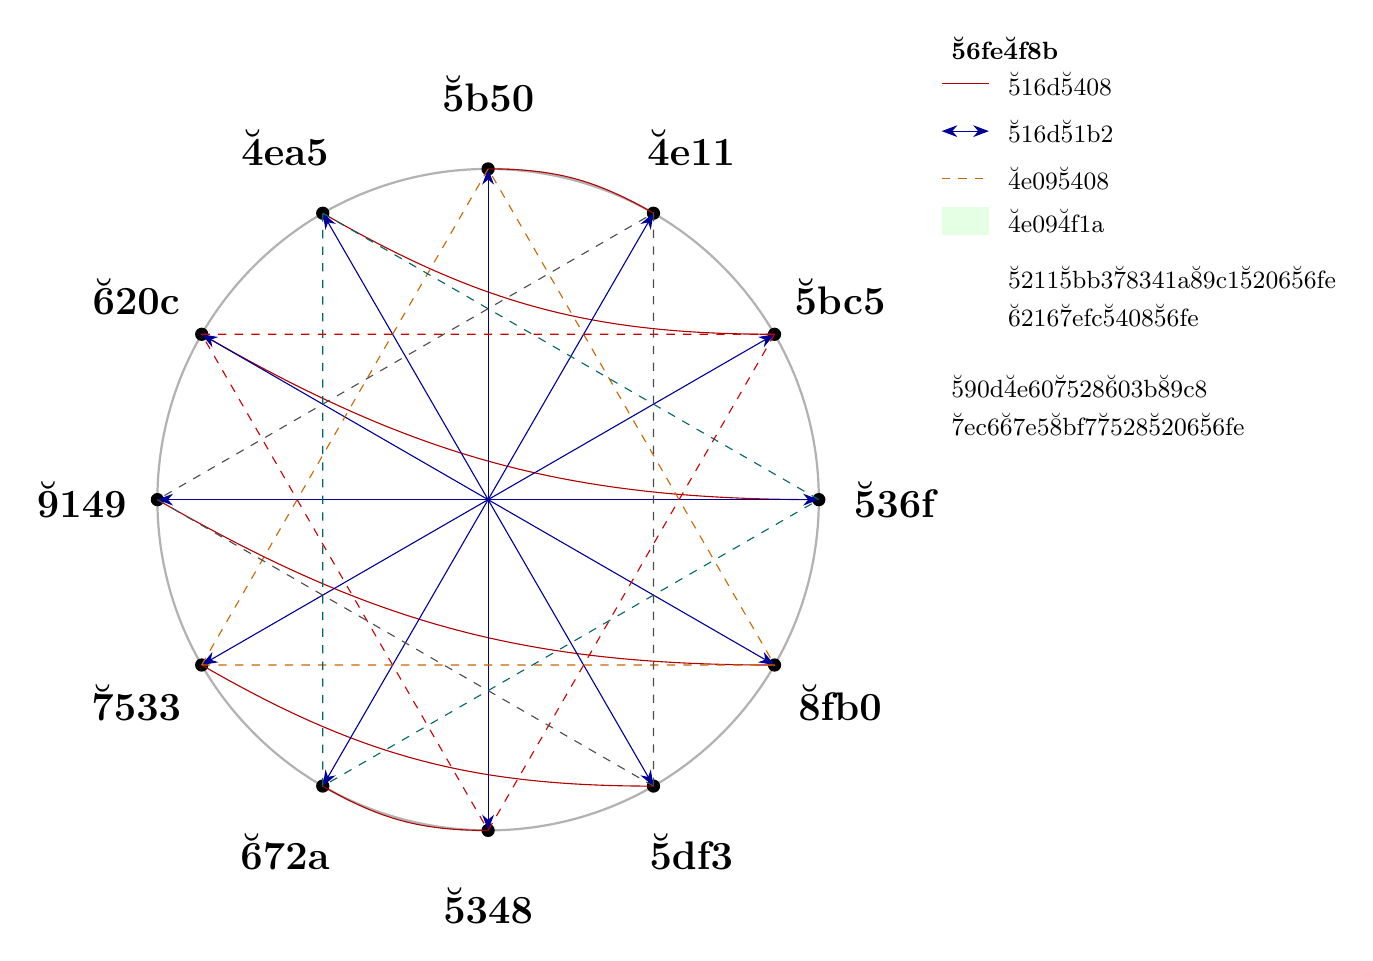
\begin{tikzpicture}[scale=1.2]
  \coordinate (zi)  at ( 90:3.5);
  \coordinate (chou) at ( 60:3.5);
  \coordinate (yin)  at ( 30:3.5);
  \coordinate (mao)  at (  0:3.5);
  \coordinate (chen) at (330:3.5);
  \coordinate (si)   at (300:3.5);
  \coordinate (wu)   at (270:3.5);
  \coordinate (wei)  at (240:3.5);
  \coordinate (shen) at (210:3.5);
  \coordinate (you)  at (180:3.5);
  \coordinate (xu)   at (150:3.5);
  \coordinate (hai)  at (120:3.5);

  \draw[thick, gray!60] (0,0) circle (3.5);

  \foreach \name/\angle/\text in {
    zi/90/\u5b50, chou/60/\u4e11, yin/30/\u5bc5, mao/0/\u536f,
    chen/330/\u8fb0, si/300/\u5df3, wu/270/\u5348, wei/240/\u672a,
    shen/210/\u7533, you/180/\u9149, xu/150/\u620c, hai/120/\u4ea5
  } {
    \fill[black] (\angle:3.5) circle (2pt);
    \node[font=\Large\bfseries] at (\angle:4.3) {\text};
  }

  % \u516d\u5408\uff1a\u7ea2\u8272\u5f27\u7ebf
  \draw[red!70!black, thin] (zi)  to[bend left=15] (chou);
  \draw[red!70!black, thin] (yin) to[bend left=15] (hai);
  \draw[red!70!black, thin] (mao) to[bend left=15] (xu);
  \draw[red!70!black, thin] (chen) to[bend left=15] (you);
  \draw[red!70!black, thin] (si)   to[bend left=15] (shen);
  \draw[red!70!black, thin] (wu)   to[bend left=15] (wei);

  % \u516d\u51b2\uff1a\u84dd\u8272\u76f4\u5f84\u7ebf
  \draw[blue!60!black, thin, {Stealth[length=2mm]}-{Stealth[length=2mm]}] (zi)  -- (wu);
  \draw[blue!60!black, thin, {Stealth[length=2mm]}-{Stealth[length=2mm]}] (chou) -- (wei);
  \draw[blue!60!black, thin, {Stealth[length=2mm]}-{Stealth[length=2mm]}] (yin)  -- (shen);
  \draw[blue!60!black, thin, {Stealth[length=2mm]}-{Stealth[length=2mm]}] (mao)  -- (you);
  \draw[blue!60!black, thin, {Stealth[length=2mm]}-{Stealth[length=2mm]}] (chen) -- (xu);
  \draw[blue!60!black, thin, {Stealth[length=2mm]}-{Stealth[length=2mm]}] (si)   -- (hai);

  % \u4e09\u5408\uff1a\u4e09\u89d2
  \draw[orange!80!black, thin, dashed] (shen) -- (zi) -- (chen) -- cycle;
  \draw[teal!80!black, thin, dashed]  (hai) -- (mao) -- (wei) -- cycle;
  \draw[red!80!black, thin, dashed]   (yin) -- (wu) -- (xu) -- cycle;
  \draw[gray!60!black, thin, dashed]  (si) -- (you) -- (chou) -- cycle;

  % \u4e09\u4f1a\uff1a\u6247\u533a\u8272\u5757
  \begin{scope}[on background layer]
    \fill[green!10]  (30:3.3) arc(30:150:3.3) -- (0,0) -- cycle;
    \fill[red!8]     (330:3.3) arc(330:30:3.3) -- (0,0) -- cycle;
    \fill[orange!8]  (210:3.3) arc(210:330:3.3) -- (0,0) -- cycle;
    \fill[blue!8]    (150:3.3) arc(150:210:3.3) -- (0,0) -- cycle;
  \end{scope}

  % \u56fe\u4f8b\uff08\u5916\u5708\u53f3\u4fa7\uff09
  \node[font=\small\bfseries, anchor=north west] at (4.8,5.0) {\u56fe\u4f8b};
  \draw[red!70!black, thin] (4.8,4.4) -- (5.3,4.4);
  \node[font=\small, anchor=west] at (5.4,4.4) {\u516d\u5408};
  \draw[blue!60!black, thin, {Stealth[length=2mm]}-{Stealth[length=2mm]}] (4.8,3.9) -- (5.3,3.9);
  \node[font=\small, anchor=west] at (5.4,3.9) {\u516d\u51b2};
  \draw[orange!80!black, thin, dashed] (4.8,3.4) -- (5.3,3.4);
  \node[font=\small, anchor=west] at (5.4,3.4) {\u4e09\u5408};
  \fill[green!10] (4.8,2.8) rectangle ++(0.5,0.3);
  \node[font=\small, anchor=west] at (5.4,2.95) {\u4e09\u4f1a};
  \node[font=\small, anchor=west] at (5.4,2.35) {\u5211\u5bb3\u7834\uff1a\u89c1\u5206\u56fe};
  \node[font=\small, anchor=west] at (5.4,1.95) {\u6216\u7efc\u5408\u56fe};
  \node[font=\small, anchor=west] at (4.8,1.2)  {\u590d\u4e60\u7528\u603b\u89c8};
  \node[font=\small, anchor=west] at (4.8,0.8)  {\u7ec6\u67e5\u8bf7\u7528\u5206\u56fe};

  % \u767d\u8272\u80cc\u666f\uff0c\u9632\u6b62 GitHub dark mode \u4e0b\u900f\u660e SVG \u770b\u4e0d\u6e05
  \begin{scope}[on background layer]
    \fill[white] (current bounding box.south west) rectangle (current bounding box.north east);
  \end{scope}
\end{tikzpicture}
\end{document}
